% file: rdt.tex

\documentclass[tikz]{standalone}

\begin{document}
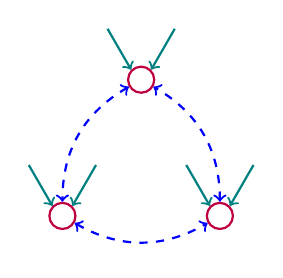
\begin{tikzpicture}[every edge/.style = {draw, <->, dashed, bend right, blue, thick},
  access/.style = {teal, <-, thick}]
  \foreach \obj/\pos in {obj1/{(0,0)}, obj2/{(2,0)}, obj3/{(1,1.73)}} {
    \node (\obj) [circle, purple, draw, minimum size = 5pt, thick] at \pos {};
    \draw[access] (\obj.north east) to +(60:0.6cm);
    \draw[access] (\obj.north west) to +(120:0.6cm);
  }

  \path (obj1) edge (obj2)
	(obj2) edge (obj3)
	(obj3) edge (obj1);
\end{tikzpicture}
\end{document}